\documentclass{article}
\usepackage[margin=4cm,includefoo t]{geometry}
\usepackage[numbers,sort&compress]{natbib}
\usepackage{graphicx} %allow for import of images
\DeclareGraphicsExtensions{.pdf,.png,.jpg}
\graphicspath{{pictures/}}
\usepackage{float}
\usepackage{amsmath}
% EQ numbering
\numberwithin{equation}{section} % do x.i equations instead of plane i
\usepackage[hidelinks]{hyperref}
\usepackage{amsfonts}
\usepackage{hyperref}
\DeclareSymbolFont{letters}{OML}{ztmcm}{m}{it} %Math font
\newcommand{\me}{\mathrm{e}}
\newcommand{\md}{\mathrm{d}}
% Signature function
\newcommand{\namesigdate}[2][5cm]{%
  \begin{tabular}{@{}p{#1}@{}}
    #2 \\[2\normalbaselineskip] \hrule \\[0pt]
    {\small \textit{Signature}} \\[2\normalbaselineskip] \hrule \\[0pt]
    {\small \textit{Date}}
  \end{tabular}
}
\usepackage{graphicx}
\usepackage{caption}
\usepackage{subcaption}
%bibliography
\usepackage[numbers,sort&compress]{natbib}

% star
\newcommand{\mystar}{{\fontfamily{lmr}\selectfont$\star$}}
% quute

\usepackage{epigraph}

% \epigraphsize{\small}% Default
\setlength\epigraphwidth{8cm}
\setlength\epigraphrule{0pt}

\usepackage{etoolbox}

\makeatletter
\patchcmd{\epigraph}{\@epitext{#1}}{\itshape\@epitext{#1}}{}{}
\makeatother

% Header and footer
\usepackage{lastpage}
\usepackage{fancyhdr}
\pagestyle{fancy}
\fancyfoot{}
\fancyfoot[R]{\thepage}
\fancyhead[LE,RO]{} 
%

%Highligth text
\usepackage{soul}
\usepackage{color}
\DeclareRobustCommand{\hlRed}[1]{{\sethlcolor{red}\hl{#1}}}
\usepackage{xcolor}
\newcommand{\highlight}[1]{%
  \colorbox{red!50}{$\displaystyle#1$}}

\begin{document}
%title page

\begin{titlepage}
	\begin{flushleft}
	\vspace*{-3.5cm}
	\hspace*{-3 cm}
		
\includegraphics[width=7cm]{pictures/Logo.png} % also works with logo.pdf
	\end{flushleft}
	\begin{center}
	\\
	[2cm]
	\textsc{\large 	Technical University of Denmark}\\
	[0.5cm]
	\textsc{\LARGE \mystar} \\
	[0.5cm]
	\textsc{\LARGE Advanced Engineering Mathematics}\\
	[2cm]
	\noindent\makebox[\linewidth]{\rule{\paperwidth}{1.5 pt}}\\
	[5mm]
	\huge{\bfseries Size structured fish populations} \\
	[0.2 cm]

	\noindent\makebox[\linewidth]{\rule{\paperwidth}{1.5 pt}}\\
	[-0.75 cm]
	\noindent\makebox[\linewidth]{\rule{\paperwidth}{0.5 pt}}\\

	\textsc{\Large}\\
	[3.5cm]
		
	\end{center}
	\begin{flushright}
	\textsc{\large Group members} \textit{Student No.}\\ 
	\line(1,0){150}\\
	Andreas Harmuth \textit{S164575} \\
	Christian E. Petersen \textit{S164568}\\
	Nicholas Rose \textit{S164580}\\
	Bosse Bandowski \textit{S164582}\\
	Jack Rose \textit{S164559}\\
	Joshua G. Whillock \textit{S165514}\\
	[1.5cm]
	\end{flushright}
	
	\begin{center}
		Date: 07/04/2017
	\end{center}
\end{titlepage}

% Before TOC

\pagenumbering{roman}
\addcontentsline{toc}{section}{\numberline{}Signature page}

\section*{Signature page}
\noindent \namesigdate{Andreas Harmuth} \hfill \namesigdate{Christian E. Petersen}\\
[3cm]
\noindent \namesigdate{Nicholas Rose} \hfill \namesigdate{Bosse Bandowski}\\
[3cm]
\noindent \namesigdate{Jack Rose} \hfill \namesigdate{Joshua Whillock}
\newpage
\addcontentsline{toc}{section}{\numberline{}Introduction}
\section*{Introduction}

This report is an in depth mathematical investigation of the size structure of fish populations. It initially studies a simple steady state model and the conservation equation for said model, and further explores the impact of fishing and optimal fishing yields, the rate at which a fish stock can recover, it answers why fish make small eggs and provides solutions to the size distribution of fish with realistic growth rates given by a von Bertalanffy growth function. \\

The mathematical solutions are heavily focused on solving differential equations and in order to make visual representations, certain constants had to be chosen. The standard constants used in this report are:
\begin{align*}
A = 5 \\
a = 0.3 \\
b = \frac{3}{4}\\
c=8 \\
\alpha =a \cdot A 
\end{align*}
These constants will be used as standard unless otherwise stated. 

This report covers all the core questions but not all the extras. The group has chosen to prioritise on deriving many of the equations and go very much in depth with the main questions. Because of this the report will \textit{not} cover question 3, extra 2. However, this does not mean it will not be prepared for in the oral exam. \\
[5cm]
\epigraph{``The essence of mathematics is not to make simple things complicated, but to make complicated things simple."}{--- \textup{S. Gudder}, Mathematician}
\newpage

\addcontentsline{toc}{section}{\numberline{}Reading guide}
\section*{Reading guide}
In this report the derivations are mostly located in the appendices. Due to this, every appendix is followed by a \textbf{Jump back} functionality. By clicking on this text you will be returned to the part which the appendix is referring to. This gives the report a better flow as looking at the appendix won't result  in the reader having to scroll back and find where he/she came from. This only works in the PDF which can be downloaded at: geneng.co/mathproject or by scanning the QR-code below.\\
\\
The CAS-tool Maple is used to support calculations and all plots and illustration is also produced in said software.\\
[5cm]
\begin{center}

\includegraphics[width=4cm]{pictures/qrcode.png}
\end{center}


\newpage

% After TOC

\cleardoublepage
%

%set pagenumbering to normal
\pagenumbering{arabic}
\fancyfoot[R]{Page \thepage\ of \pageref{LastPage}}
%table of content
\listoffigures
\listoftables
\thispagestyle{empty} %remove page number
\newpage
\thispagestyle{empty} %remove page number
\tableofcontents 
\thispagestyle{empty} %remove page number
\cleardoublepage
\setcounter{page}{1}
%


%Exercise 1
\section{Solving the conservation equation}\label{sec:Ex1}
The abundance is the distribution of fish in a given size group. It can be expressed as both a function of size but also as a function of both size and time. This section doesn't concerns itself with the latter. To find said function one must derive from the differential equation given in the exercise:\\
\\
The conservation equation can be solved as a differential equation given the following information:
\begin{equation}\label{eq:alphaaa}
	\alpha = a \cdot A
\end{equation}
and,
\begin{equation}
	b = \dfrac{3}{4}
\end{equation}
The function $\mu$, then becoms,
\begin{equation}\label{eq:Ex1mu}
	\mu (x) = \alpha x^{b-1} = aAx^{\tfrac{3}{4}-1}
\end{equation}
Similarly, the equation for $g$ can be expressed as:
\begin{equation}\label{eq:Ex1g}
	g(x) = Ax^{b-1} =Ax^{\tfrac{3}{4}}
\end{equation}
From substituting the expression \ref{eq:Ex1mu} and \ref{eq:Ex1g} for $\mu$ and $g$ the differential equation can be stated:
\begin{equation}
	\dfrac{\md Ax^{\tfrac{3}{4}}n(x)}{\md x} = -aAx^{\tfrac{3}{4}-1}n(x)
\end{equation}
Solving this equations for $n(x)$ yields the result:
\begin{equation}\label{eq:Ex1n}
	n(x) = cx^{-\tfrac{3}{4}-a} \qquad \textrm{where } c \in \mathbb{R}
\end{equation}
The derivation can be found in \hyperref[a:calcEx1a]{Appendix \ref{a:calcEx1a}}\label{jmp:a:calcEx1a}
%Section 1.1
\subsection{Plot of the abundance distribution and biomass}\label{sec:Ex1A}
The abundance distribution and biomass is plotted in \hyperref[fig:e1p12]{figure \ref{fig:e1p12}} with a constant a-value of 0.3 as well as c-values of 5, 10 and 20 to show the difference. Biomass is furthermore plotted as a function of x and c which can be found in \hyperref[a:biomassPlot]{Appendix \ref{a:biomassPlot}}\label{jmp:a:biomassPlot}
\begin{figure}[t!]
 
\begin{subfigure}[t]{0.5\textwidth}
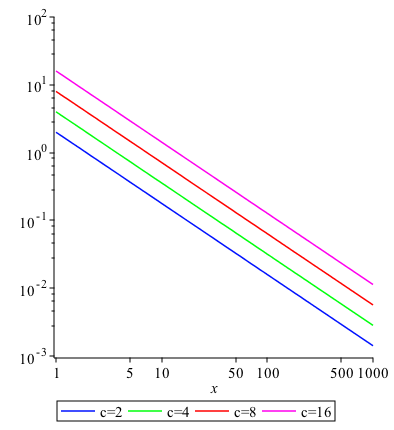
\includegraphics[width=0.9\linewidth]{exercises/e1p1} 
\caption{Abundance distribution given different c-values in a log-plot}

\end{subfigure}
\begin{subfigure}[t]{0.5\textwidth}
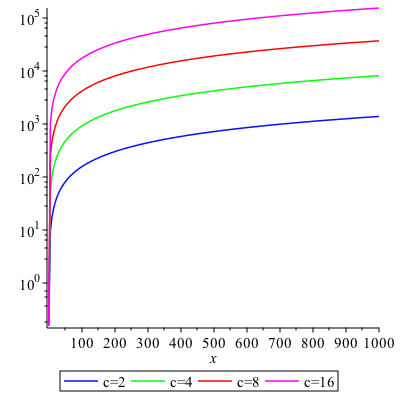
\includegraphics[width=0.9\linewidth]{exercises/e1p2}
\caption{Biomass given different c-values in a semilog-plot (y-axis)}
\label{fig:e1p2}
\end{subfigure}
\caption{Plot of the abundance distribution and biomass respectively. The different coloring corresponds to the following c-values: blue;2, green;4, red;8, purple;16. Both plots have an a-value of 0.3} 
\label{fig:e1p12}
\end{figure}
\newpage

\subsection{Investigation of biomass}\label{sec:Ex1B}
The biomass will be investigated for the c-values 2,4,8,16. The equation for biomass can be found in \hyperref[a:biomassPlot]{Appendix \ref{a:biomassPlot}}\ equation \ref{eq:biomass2v}. For the different c-values it yields:\\
\begin{table}[h!]
    \centering
    \begin{tabular}{ |p{2.4cm}||p{2.4cm}|p{2.4cm}|p{2.4cm}|p{2.4cm}|  }
     \hline
     \multicolumn{5}{|c|}{Biomass at different values of c and x} \\
     \hline
     \textbf{c-values/x-values}& \textbf{x=100} &\textbf{x=300}&\textbf{x=600}&\textbf{x=1000}  \\
     \hline
     \hline
     \textbf{c=2}   & 155.83  &442.52& 854.88 & 1388.87\\
     \hline
     \textbf{c=4} &   913.77  & 2594.80 & 5012.82 & 8144.01\\
     \hline
     \textbf{c=8} & 4153.92 & 11795.69 & 22787.78 & 37021.86\\
     \hline
     \textbf{c=16}& 17296.37 & 49115.67& 94885.22 & 1.54\cdot10^5\\
     \hline
    \end{tabular}
    \caption{Biomass given at different c and x values}
    \label{tab:biomass2v}
\end{table}\\
The c-values double for each time. As it is seen here, the biomass depends heavily on the c-values. The factor between the biomass of a c-value and the biomass at the same x-value but given a c-value twice as large is approximately:
\begin{equation}
    \dfrac{4c_{small}-2}{c_{small}-1}
\end{equation}
The derivation of the approximation is found in \hyperref[a:biomassDifApprox]{Appendix \ref{a:biomassDifApprox}}\label{jmp:a:biomassDifApprox}. Here $c_{small}$ corresponds to the smallest value. A doubling from 2 to 4 will give a yield 6 times as big. This is in accordance with the values in \hyperref[tab:biomass2v]{table \ref{tab:biomass2v}}. As the c-number rises, the difference in yields decreases towards one-forth of the initial difference. (see \hyperref[a:sub:largeCvalues]{Appendix \ref{a:sub:largeCvalues}} ).


%Exercise 2
\section{What is the biomass of a cohort of fish?}\label{sec:Ex2}
A cohort of fish is a collection of fish that is born in the same group or batch. Under the assumption that a cohort is born in a small time interval $\Delta$t, the mass of the cohort shall be found.

\subsection{Investigation of the cohort biomass}\label{sec:Ex2A}
The mass of the cohort is given by,
\begin{equation}\label{eq:CohortIntegral}
  c(x) = \int_{x}^{x+\dfrac{\md x(t)}{\md t}\cdot\Delta t} n(\xi)\cdot\xi d\xi
\end{equation}
Similarly, this can also be approximated by:
\begin{equation}\label{eq:apprCohortBiomass}
	c(x)=n(x)x\dfrac{\md x(t)}{\md t}\Delta t
\end{equation}
The proof of this approximation can be found in \hyperref[a:proofBiomassCohort]{Appendix \ref{a:proofBiomassCohort}} along with the step-by-step solution of the integral in equation \ref{eq:CohortIntegral}. From \hyperref[a:proofBiomassCohort]{Appendix \ref{a:proofBiomassCohort}}\label{jmp:a:proofBiomassCohort}, the following solution was obtained.
\begin{equation}\label{eq:e2integralsolution}
    c(x) = \left[\dfrac{c\cdot\xi^{(\tfrac{1}{4}-a)+1}}{\tfrac{1}{4}-a+1}\right]_x^{x+\tfrac{\md x(t)}{\md t}\Delta t} = \left[\dfrac{c\cdot\xi^{(\tfrac{5}{4}-a)}}{\tfrac{5}{4}-a}\right]_x^{x+\tfrac{\md x(t)}{\md t}\Delta t}
\end{equation}
\begin{figure}
    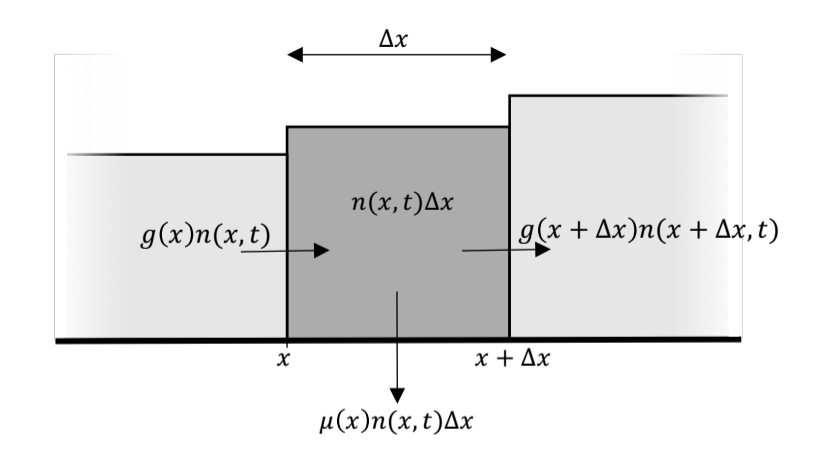
\includegraphics[width=0.9\linewidth]{exercises/ex2_balance}
    \caption{Sketch of balance between growth and mortality in a group}
    \label{fig:Balance}
\end{figure}
From figure \ref{fig:Balance}, the balance between growth and mortality in a group can be written as,
\begin{equation}
    n(x,t)\Delta x + g(x)n(x,t)-\mu (x)n(x,t)\Delta x -g(x+\Delta x)n(x+\Delta x,t)
\end{equation}
The change in size for fish can also be considered the growth rate, hence, $\dfrac{dx(t)}{dt}$ can be expressed as g(x) and equation \ref{eq:e2integralsolution} becomes,
\begin{equation}
    \left[\dfrac{c\cdot\xi^{(\tfrac{5}{4}-a)}}{\tfrac{5}{4}-a}\right]_x^{x+g(x)\Delta t}
\end{equation}
By substituting the limits, the final function can then be evaluated as,
\begin{equation}\label{eq:e2biomass}
    	c(x)=\left(
	    \dfrac{c\cdot\left(
	        x+g(x)\cdot\Delta t
	    \right)^{\tfrac{5}{4}-a}}{\tfrac{5}{4}-a}
	\right)-\left(
	    \dfrac{cx^{\tfrac{5}{4}-a}}{\tfrac{5}{4}-a}
	\right)
\end{equation}
Similarly, the approximation is given by,
\begin{equation}\label{eq:e2approximation}
c(x)=2\cdot\dfrac{A\cdot x^{b}\cdot \Delta t}{x^{0.05}}
\end{equation}
To check how biomass changes with respect to time c(x(t)), it is necessary to solve for x(t). It was previously determined that g(x) = $\dfrac{dx(t)}{dt}$. Therefore, 
\begin{equation}
    \dfrac{dx(t)}{dt}=Ax^{b}
\end{equation}
This is an easily solved differential equation. Firstly  match the variables with x(t) on the left hand side and t on the right hand side. 
\begin{equation}\label{eq:e2diff}
    \dfrac{dx(t)}{x^{b}}=Adt
\end{equation}
Now setting up the integrals,
\begin{equation}\label{eq:e2integrals}
    \int\frac{1}{x^{b}}dx(t)=\int Adt
\end{equation}
Assuming that b $\neq$ 1, The normal power rule is applied and equation \ref{eq:e2integrals} becomes,
\begin{equation}
    \frac{x^{-b+1}}{-b+1}=At+c
\end{equation}
Solving for x,
\begin{equation}\label{eq:e2x(t)}
    x(t)=((At+c)(-b+1))^{\frac{1}{1-b}}
\end{equation}
For graphing purposes, certain constants were chosen,
\begin{equation}\label{eq:e2constants}
c=2 \qquad a=0.3 \qquad  b=\dfrac{3}{4} \qquad \alpha=1
\end{equation}
From equation \ref{eq:alphaaa},  the substitution $A = \frac{\alpha}{a}$ can be made and the final equation for x(t) becomes.
\begin{equation}\label{eq:finalxt}
    x(t)=\left(\frac{10}{3}t+\frac{1}{2}\right )^{4}
\end{equation}
Lastly, the final cohort masses are given as follows,
\begin{equation}\label{eq:cex}
    c(x(t))_{exact}= \frac{20}{3}\, \left(  \left(  \frac{10}{12}\,t+1/2 \right) ^{4}
 \right) ^{\frac{7}{10}}t
\end{equation}
\begin{equation}\label{eq:capp}
    c(x(t))_{approx}=\frac{20}{3}\, \left(  \left(  \frac{10}{12}\,t+1/2 \right) ^{4}
 \right) ^{- \frac{3}{10}} \left(  \frac{10}{12}\,t+1/2 \right) ^{4}t
\end{equation}
The functions \ref{eq:cex} and \ref{eq:capp} were plotted in figure \ref{fig:ex2}. It is seen that the approximation follows the exact solution very closely, and deviates slightly at larger values of x. It appears that cohort mass with respect to x(t) increases forever from these plots. This is because it fails to factor in various real life variables, including mortality and fishing, these aspects will be covered later in this report.
\begin{figure}
\begin{subfigure}{0.5\textwidth}
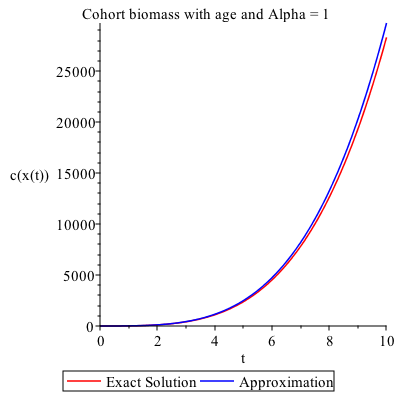
\includegraphics[width=0.9\linewidth]{exercises/ex2_Approx-vs-Exact-age} 
\caption{The approximation and the exact function for cohort biomass with age}

\end{subfigure}
\begin{subfigure}{0.5\textwidth}
\centering
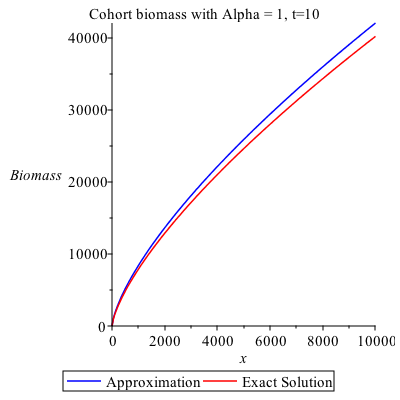
\includegraphics[width=0.9\linewidth]{exercises/ex2_Approx-vs-Exact-Size}
\caption{The approximation and the exact function for cohort biomass with size}
\label{fig:ex2age}
\end{subfigure}
\caption{Plots of cohort biomass with respect to age and size.} 
\label{fig:ex2}
\end{figure}
\newpage




%Exercise 3
\section{Now add fishing}\label{sec:Ex3}
It is obvious that the fish mortality rate is dependent on how much fishing activity the stocks are exposed to. This amount of fishing is a constant given by $\alpha_F$. The mortality depends on this constant in the following way:

\begin{equation}
\mu(x) =
       \left\{
        \begin{array}{ll}
              \alpha x^{b-1} & x_0 < x < x_F \\
              (\alpha+\alpha_F) x^{b-1} &  x\geq x_F \\
        \end{array} 
\right.
\end{equation}
Following this function, one can calculate (found in \hyperref[a:abundancepiecewise]{Appendix \ref{a:abundancepiecewise}}\label{jmp:a:abundancepiecewise}) the abundance as a piece wise function as well:

\begin{equation}\label{eq:ex3nx}
    n(x) =
       \left\{
        \begin{array}{ll}
              cx^{-b-a} & x_0 < x < x_F \\
              x_F^{a_F}cx^{-b-a-a_F} & x_F\leq x \\
        \end{array} 
\right.
\end{equation}
These two functions are illustrated in figure \ref{fig:ex3double}:


\begin{figure}[h]
\begin{subfigure}{0.5\textwidth}
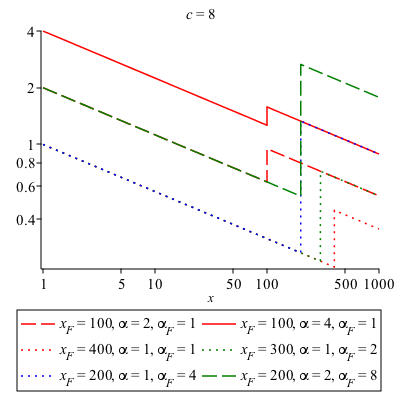
\includegraphics[width=0.9\linewidth]{exercises/ex3p1} 
\caption{Piecewise function of $\mu(x)$ when taking fishing into account}

\end{subfigure}
\begin{subfigure}{0.5\textwidth}
\centering
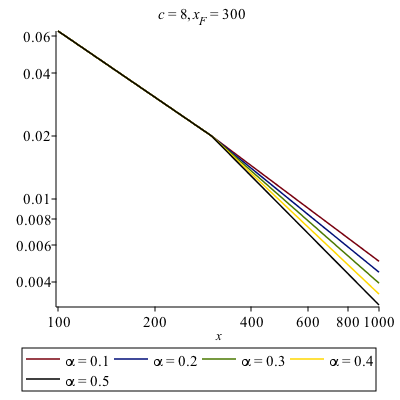
\includegraphics[width=0.9\linewidth]{exercises/ex3p2}
\caption{Piecewise function of $n(x)$ when taking fishing into account}
\end{subfigure}
\caption{A plot showing how fishing affects the mortality and abundance} 
\label{fig:ex3double}
\end{figure}
As expected, a high fishing constant corresponds to a higher mortality and thereby a lower abundance. This is very important when looking at the yield when fishing and how to optimize it. The rest of this chapter will  focus on the yield.

\subsection{Yield from the fishery}\label{sec:Ex3A}
The yield from the fishery is the similar to the biomass but multiplied with the amount of fishing inside the integral. Therefore it becomes an integral of the amount of biomass that is being fished:

\begin{equation}\label{eq:yieldsnx}
    \int_{x_F}^{x_\infty}n(x)x\alpha_Fx^{b-1}\md x
\end{equation}
Substituting n(x) when one is fishing in \hyperref[eq:yieldsnx]{equation \ref{eq:yieldsnx}} gives:

\begin{equation}\label{eq:ex3yield}
    \int_{x_F}^{x_\infty}x_F^{a_F}cx^{-b-a-a_F}x\alpha_Fx^{b-1}\md x
\end{equation}
Treating the above as a function, one can plot it in 3d where the variables are $x_F$ and $\alpha_F$. As usual the following constants are used:

\begin{align}
    a = 0.3\\
    b = \dfrac{3}{4}\\
    c = 8
\end{align}
With an $x_{\infty}$-value of 1000 the plotted function (derivation in \hyperref[a:yieldFunction]{Appendix \ref{a:yieldFunction}})\label{jmp:a:yieldFunction} becomes:

\begin{equation}%do a function instead of the integral
	Y(x_F,\alpha_F) = \dfrac{80\alpha_F\left(x_F^{7/10}-125.89\exp(-6.9078\alpha_F)x_F^{\alpha_F}\right)}{10\alpha_F-7}
\end{equation}
This function is plotted beneath in 3d,
\begin{figure}[h]\label{fig:ex3p3a4}
    \begin{subfigure}[t!]{0.5\textwidth}
        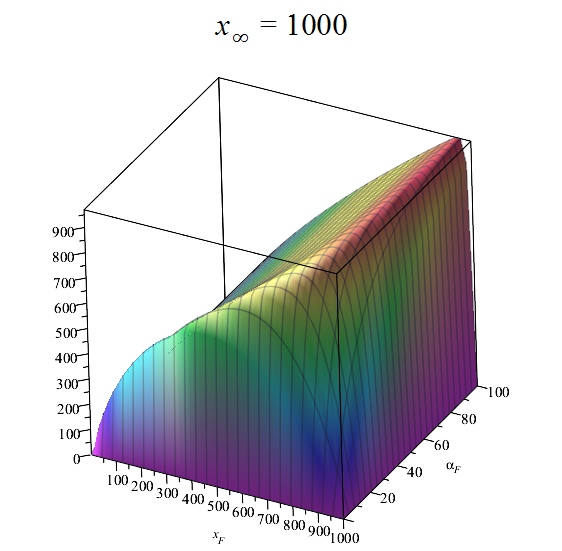
\includegraphics[width=0.9\linewidth]{exercises/ex3p3} 
        \caption{3d-plot of the yield as a function of $x_F$ and $\alpha_F$}
        \label{fig:ex3p4}
    \end{subfigure}
\begin{subfigure}[t!]{0.5\textwidth}
        \centering
        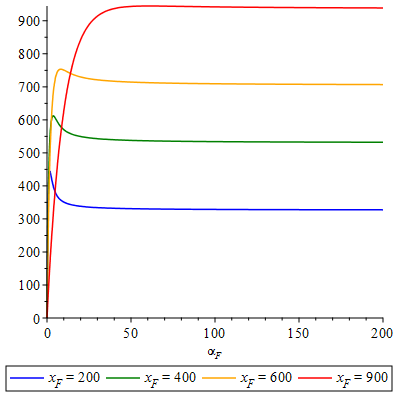
\includegraphics[width=0.9\linewidth]{exercises/ex3p4}
        \caption{Plots of yield with different constant starting sizes }
    \end{subfigure}
    \caption{Plots of yield with different constant starting sizes, $x_F$} 
    \label{fig:ex3p4}
\end{figure}

The plot shows that to get the maximum yield one has to fish as much as possible and as heavy fish as possible; the maximum yield is thereby given when $x$ is infinitely close to $x_\infty$ and $\alpha_F$ is as large as possible. This is proven in \hyperref[a:fishingStrategy]{Appendix \ref{a:fishingStrategy}}\label{jmp:a:fishingStrategy}. So how does this make sense? In the real world one can not keep fishing infinitely hard on all the grown fish and expect to get the largest yield. Clearly something is wrong with this model. And yes, there is. It's not incorrect per se; it just lacks one important factor. It assumes that there are infinitely many fish. And given this assumption the answer found in this section seems very plausible. Later this report will look at the situation where this assumption is incorrect. 

\subsection{Fishing with a fishing mortality that is constant with size}\label{sec:Ex3extra1}
In the calculations above the fishing mortality was depended on the size. However, in this subsection the fishing mortality is constant with size. This constant is denoted $\mu_F$. One can then describe fishing mortality as the following:

\begin{equation}
\mu(x) =
       \left\{
        \begin{array}{ll}
              \alpha x^{b-1} & x_0 < x < x_F \\
              \alpha x^{b-1}+\mu_F &  x\geq x_F \\
        \end{array} 
\right.
\end{equation}
One can then derive the abundance (which is shown in \hyperref[a:3extra1nx]{Appendix \ref{a:3extra1nx}})\label{jmp:a:3extra1nx} as:

\begin{equation}\label{eq:ex3extranx}
    n(x) =
       \left\{
        \begin{array}{ll}
              cx^{-b-a} & x_0 < x < x_F \\
              \exp\left(\dfrac{\mu_F\left(-x_F^{-b+1}+x^{-b+1}\right)}{A(b-1)}\right)x^{-a-b}c & x_F\leq x \\
        \end{array}
\right.
\end{equation}
From this the yield is given in the same way as \hyperref[eq:yieldsnx]{equation \ref{eq:yieldsnx}}. By substituting the function for n(x) when $x\geq x_F$  in \hyperref[eq:yieldsnx]{expression \ref{eq:yieldsnx}}  the yield becomes:

\begin{equation}\label{yeildExtra}
    \begin{split}
        Y(x_F,\mu_F) &= \int_{x_F}^{x_\infty}\left(\dfrac{\mu_F\left(-x_F^{-b+1}+x^{-b+1}\right)}{A(b-1)}\right)x^{-a-b}c\mu_F x\md x\\
    	&=c\mu_F\int_{x_F}^{x_\infty}\left(\dfrac{\mu_F\left(-x_F^{-b+1}+x^{-b+1}\right)}{A(b-1)}\right)x^{1-a-b}\md x
    \end{split}
\end{equation}
Below on \hyperref[fig:ex3p4]{figure \ref{fig:ex3p4}} is the new function for yield on top of the original function. It is clear that the yield becomes more \textit{aggressive} and higher. The reason for the higher yield is based on the fact that the mortality rate doesn't depend on the size anymore. Bigger fish don't tend to die more. This is why this model is much more aggressive. The blue model (which depends on fishing size) flattens out much quicker for that exact reason. 

\begin{figure}[t]
    \begin{subfigure}[t]{0.5\textwidth}
        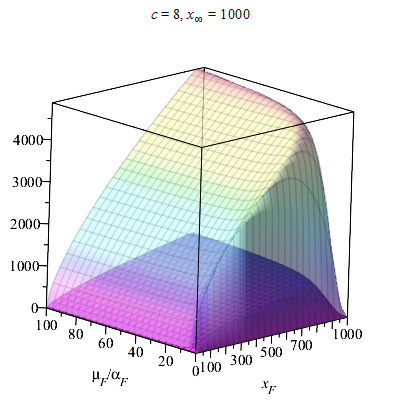
\includegraphics[width=0.9\linewidth]{exercises/ex3ep1} 
        \caption{3d-plot of the yield as function of $x_F$ and $\mu_F$ (Hue color) on top of the yield as a function of $x_F$ and $\alpha_F$ (Blue)}
    \end{subfigure}
\begin{subfigure}[t]{0.5\textwidth}
        \centering
        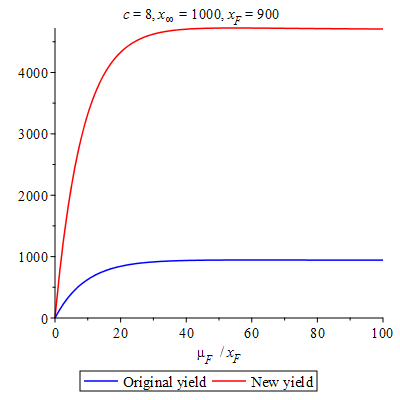
\includegraphics[width=0.9\linewidth]{exercises/ex3ep2}
        \caption{\textbf{2d-plot of the yield as function of $x_F$ and $\mu_F$ (red) on top of the yield as a function of $x_F$ and $\alpha_F$ (blue). Here $x_F$ is held constant at 900}}
    \end{subfigure}
    \caption{Plots of the difference between having a yield function of $\mu_F$ compared to $\alpha_$} 
    \label{fig:ex3p4}
\end{figure}
\newpage
%Exercise 4
\section{How fast can a fish stock recover?}\label{sec:Ex4}
Once a fish stock has been overfished and is depleted, it needs time to recover. The progress of recovery depends on the reproductive output, the population growth rate and the mortality and growth coefficients that have been introduced earlier (A, $\alpha$ , $\alpha_F$,  b). Unless stated otherwise, the following standard values for these coefficients from the exercise set are used:

\begin{align}
    \alpha = 1.5\\
    \alpha_F = 0
\end{align}
 $\alpha_F$ is set to be 0. Since the fish stock is recovering, it is assumed that very little to no fishing activity is going on.

\subsection{Finding an expression for the population growth rate}\label{sec:Ex4A}
So far, time has not been an important factor in the calculations. This has to change now if one wants to model the recovery of fish stocks. To introduce time, one can rewrite the abundance function \textit{n} as:

\begin{equation}\label{eq:givennx}
	n(x,t)=\me^{rt}f(x)
\end{equation}

This assumes that the abundance develops exponentially over time depending on the population growth rate r and a size distribution f(x). The equation for conservation is given by:

\begin{equation}\label{eq:conservationPartial}
	\dfrac{\partial n(x,t)}{\partial t} + \dfrac{\partial g(x)n(x,t)}{\partial x} = \mu(x)n(x,t)
\end{equation}
Inserting the expression from \hyperref[eq:givennx]{equation \ref{eq:givennx}} into the conservation equation as seen in allows us to solve for f(x) which is shown in \hyperref[a:derivation_fx]{Appendix \ref{a:derivation_fx}}\label{jmp:a:derivation_fx}:

\begin{equation}\label{eq:fxcalculated}
	f(x) = cx^{-b-a-a_F}\exp\left(\tfrac{x^{-b+1}r}{A(b-1)}\right)
\end{equation}
Comparing the solution for f(x) to the original function $n_{init}(x)$, it is easy to spot that f(x) can be rewritten as: 

\begin{equation}
    f(x)=n_{init}\exp\left(\dfrac{x^{1-b}r}{A(b-1)}\right)
\end{equation}
It is simply the initial function multiplied by another term. This extra term accounts for the factor $\me^{rt}$ which f(x) is multiplied with to form n(x, t):

\begin{equation}
    n(x,t)= n_{init}\me^{\tfrac{x^{1-b}r}{A(b-1)}}\me^{rt}
\end{equation}

The given reproductive output, \textit{R}, and its boundary condition to the conservation equation allow one to set up an equation and solve it to find an expression for the growth rate r (this is derived in \hyperref[a:derivation_r]{Appendix \ref{a:derivation_r}}\label{a:derivation_r}):

\begin{equation}\label{eq:rfunc}
	r(x_0,x_m) = \dfrac{ln\left( x_m^{\tfrac{A-\alpha-\alpha_F}{A}}\epsilon x_0^{-\tfrac{A-\alpha-\alpha_F}{A}}\right)A(b-1)}{-x_m^{-b+1}+x_0^{-b+1}}
\end{equation}
As one can see, r depends on the growth and mortality coefficients as well as the initial size of the offspring $x_0$ and the mature size $x_m$. Below is a 3d plot of r of the latter variables in both 3d as well as 2d:
\begin{figure}[h]
\begin{subfigure}[t]{0.5\textwidth}
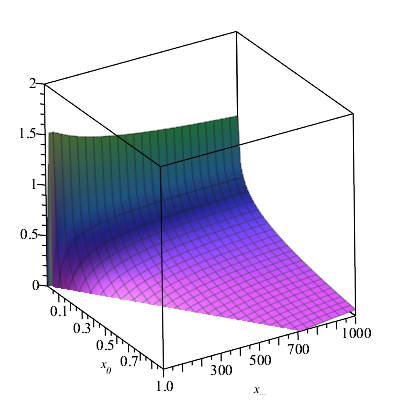
\includegraphics[width=0.9\linewidth]{exercises/ex4p1} 
\caption{The population growth rates as a function of $x_m$ and $x_0$}

\end{subfigure}
\begin{subfigure}[t]{0.5\textwidth}
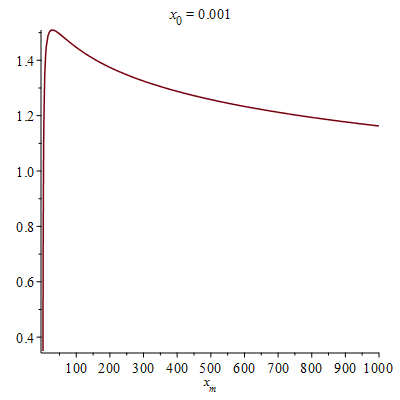
\includegraphics[width=0.9\linewidth]{exercises/ex4p2}
\caption{The population growth rates as a function of $x_m$ with a constant $x_0 = 0.001$}
\label{fig:e1p2}
\end{subfigure}
\caption{Plots of the population growth rates both in 3d and 2d} 
\label{fig:e1p12}
\end{figure}

Using $x_0=0.001$ which is introduced in part 5) of the exercise set, it is possible to give an estimate of the population growth rates of different species, e.g. herring ($x_m=100$) and cod ($x_m=10000$)

\begin{align}
    r_{Herring} = r(0.001,100) = 1.45\label{eq:r_herring_val}\\
    r_{Cod} = r(0.001,10000) = 0.850\label{eq:r_cod_val}
\end{align}

Knowing the population growth rates for these species gives the opportunity to actually estimate their recovery times. In this specific case, we are interested in knowing how much time it takes for these fish to recover a factor of 10 in biomass. The biomass is given by:

\begin{equation}
	\int_{x_1}^{x_2}n(x,t)x\md x
\end{equation}
The initial condition expressed mathematically yields the following equation (given \hyperref[eq:givennx]{equation \ref{eq:givennx}} and \hyperref[eq:fxcalculated]{equation \ref{eq:fxcalculated}}):

\begin{equation}
	\int_{x_0}^{x_m}10\me^{r0}cx^{-b-\tfrac{\alpha}{A}-\tfrac{\alpha_F}{A}}\exp\left(\tfrac{x^{-b+1}r}{A(b-1)}\right)x\md x = \int_{x_0}^{x_m}\me^{rt}cx^{-b-\tfrac{\alpha}{A}-\tfrac{\alpha_F}{A}}\exp\left(\tfrac{x^{-b+1}r}{A(b-1)}\right)x\md x
\end{equation}
Solving this equation for the time t gives

\begin{equation}\label{eq:solvet}
	t = \dfrac{ln(10)}{r}
\end{equation}
One can insert the population growth rates for herring and cod found in \hyperref[eq:r_herring_val]{equation \ref{eq:r_herring_val}} and \hyperref[eq:r_cod_val]{equation \ref{eq:r_cod_val}} to find an estimate for the recovery time t:

\begin{align}
    t_{Herring} = \dfrac{ln(10)}{1.45} = 1.59\\
    t_{Cod} = \dfrac{ln(10)}{0.850} = 2.71
\end{align}

Note that the unit of this result depends on the units of the input arguments. Thus, it is not easy to express the recovery times in months or years, but it is possible to conclude that big fish have a longer recovery time than small ones.

\subsection{The smallest viable adult size $x_m$}\label{sec:Ex4B}
As stated in \hyperref[sec:Ex4A]{section \ref{sec:Ex4A}}, the population growth rate r depends on both the initial size $x_0$ and the adult size $x_m$. The smallest viable adult size $x_m$ can be found by setting $r=0$ and solving for $x_m$. With a variable $x_0$, $x_{m_{min}}$ (x-m--min) can be expressed as a linear function of $x_0$:

\begin{equation}\label{eq:req0_1}
	x_{m,min}(x_0)=\exp\left(\dfrac{(A-\alpha-\alpha_F)ln(x_0)-ln(\epsilon)A}{A-\alpha-\alpha_F}\right)=0
\end{equation}
Inserting the standard coefficients one can obtain the solution:

\begin{equation}
	x_m = 719.69x_0
\end{equation}
This is linear relationship is shown below:
\begin{figure}[h!]
\centering
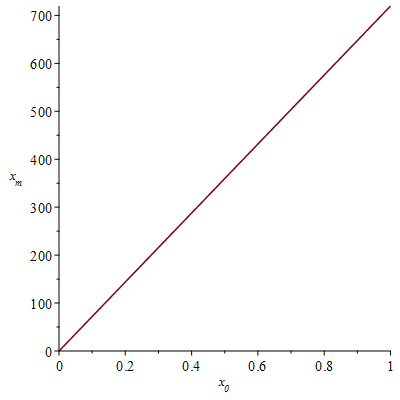
\includegraphics[width=.75\textwidth]{exercises/ex4p3}
	\caption{Plot of $x_m$ as a function of $x_0$}
	\label{fig:linrelxmx0}
\end{figure}\\
One can now easily insert a value for $x_0$. In this case the value of 0.001 is used:
\begin{equation}
	x_m = 719.69\cdot0.001 = 0.720
\end{equation}
This result is surprisingly small and not very realistic. This is probably due to the fact that the coefficients that led to this result are not specific for one species but rather arbitrary. One can however conclude that the minimum viable adult size is highly dependent on the size of the offspring. The smaller $x_0$, the smaller $x_m$. This is further investigated in part 5) of this report.
\subsection{The maximum fishing pressure}\label{sec:Ex4C}
In order to find the maximum fishing pressure, one can use a similar approach as in \hyperref[sec:Ex4B]{section \ref{sec:Ex4B}}. Setting r=0 and solving for $\alpha_F$ yields a three-dimensional function for $\alpha_{F_{max}}$ of $x_0$ and $x_m$. This is the same equation as \hyperref[sec:Ex4B]{equation \ref{eq:req0_1}} except that $\alpha_F$ is not a constant - it is the function one is solving for:

\begin{equation}
	\dfrac{ln\left( x_m^{\tfrac{A-\alpha-\alpha_F}{A}}\epsilon x_0^{-\tfrac{A-\alpha-\alpha_F}{A}}\right)A(b-1)}{-x_m^{-b+1}+x_0^{-b+1}} = 0
\end{equation}
Solving for $\alpha_F$ with the standard values yields the function: 

\begin{equation}
    \alpha_f(x_0,x_m)=\dfrac{7(ln(x_0)-ln(x_m))+46.05}{2(ln(x_0)-ln(x_m))}
\end{equation}
This function is plotted below:

\begin{figure}[H]
\centering
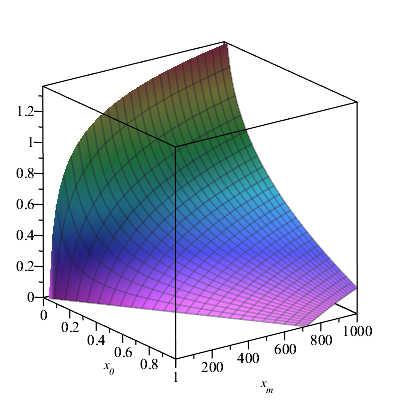
\includegraphics[width=.6\textwidth]{exercises/ex4p4}
	\caption{Plot of the the maximum $\alpha_f$ given r=0}
	\label{fig:ex4p4}
\end{figure}\\

The maximum fishing pressure $\alpha_{F_{max}}$ can be found by inserting the corresponding values for $x_0$ and $x_m$. In general, on can say that the bigger the difference between $x_m$ and $x_0$, the bigger the maximum fishing pressure. For example, the maximum fishing pressure that herring can withstand is 1.5 whereas for cod it is 2.07.
\newpage
%Exercise 5
\section{Why do fish make small eggs?}\label{sec:Ex5}
Fish are very abnormal in their way of reproducing. They size of their eggs does not correspond logically to the size of the grown-up fish. The subsection tries to explain the mathematical principles the size of the eggs. 

\subsection{Survival change of eggs}
The survival chance of an egg is given by:

\begin{equation}
    P_{x_0\rightarrow x} = \exp\left[{-\int_{x_0}^{x}\tfrac{\mu(x)}{g(x)}\md x}\right]
\end{equation}
This can be written as (derivation in \hyperref[a:survivalDerivation]{Appendix \ref{a:survivalDerivation}})\label{jmp:a:survivalDerivation}:

\begin{equation}\label{eq:survivalfinal}
    P(x_0,x) = \me^{a(ln(x_0)-ln(x))}
\end{equation}
To visualise this function it is plotted in 3d with a $\alpha$-value of 0.3:

\begin{figure}[H]
\centering
    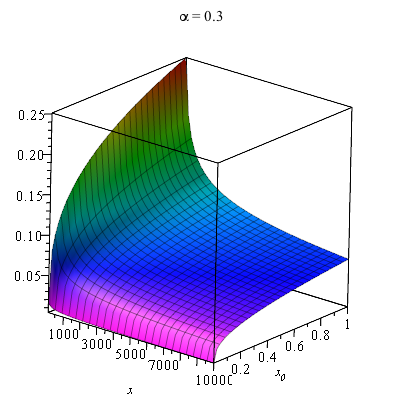
\includegraphics[width=.6\textwidth]{exercises/ex5p1.png}
    \caption{3d-plot of function \ref{eq:survivalfinal} in the range $x \in [100,10000] and x_o \in [0.0001,1] $}
    \label{fig:a2p1}
\end{figure}
The plots show the survival chance of the egg. It is made in a z-hue-coloring to support the following statements; 
\begin{itemize}
  \item The larger the grown-up fish is, the lower chance the egg has to survive.
  \item The larger the egg is, the higher change it has of surviving
\end{itemize}
Now one would expect all fish to just lay very big eggs. However, it is not quite this simple. The reason for this can be read in the subsection below.
\subsection{Sometimes quantity is better than quality}\label{sec:Ex5A}
Previously,  it was stated the bigger eggs have a bigger chance of survival. This begs the question: "Why do they then produce small eggs?" The answer lies in the question the amount of eggs that's being produces. This 'amount' can be expressed as the energy going into growth divided by the growth:
\begin{equation}
    reproduction = \dfrac{g(x)}{x_0}
\end{equation}
Now instead of looking at a single egg one should look at the group of eggs given by the reproduction. The survival is still the same as it is a factor. Because of this, the amount of eggs that survive is simply the product of the survival chance and the reproduction. This yields a function which is denoted "fitness":
\begin{equation}\label{eq:fitness}
    fitness(x_0,x) = \me^{a(ln(x_0)-ln(x))}\cdot\dfrac{g(x)}{x_0}
\end{equation}
 Below is the 3d graph as well as a 2d graph where x is constant at 100000 ~ the weight of a cod:
\begin{figure}[H]
\begin{subfigure}[t]{0.5\textwidth}
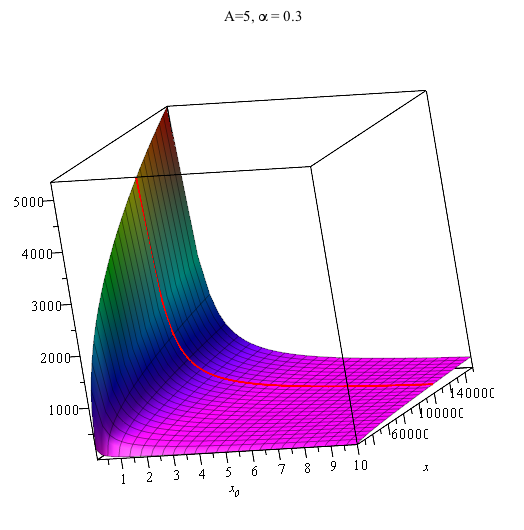
\includegraphics[width=0.9\linewidth]{exercises/ex5p21} 
\caption{3d-plot of the fitness-level. The red line is the fitness-level of the eggs from a cod, where the x value is constant at 100000}

\end{subfigure}
\begin{subfigure}[t]{0.5\textwidth}
\centering
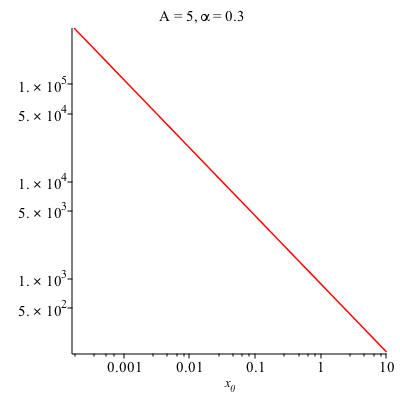
\includegraphics[width=0.9\linewidth]{exercises/ex5p22}
\caption{\textbf{The fitness level of the eggs from a cod. Here the x value is held constant at 100000.This plotted in the double logarithm scale.}}
\label{fig:ex5p21}
\end{subfigure}
\caption{Plots fitness levels in both 3d and 2d} 
\label{fig:ex5p21}
\end{figure}
The interpretation of this plot is that producing smaller eggs maximises the amount of fish reaching a grown-up state. This might seem counter-intuitive as it was previously stated the survival change of an egg increased heavily with size. However, by one is not looking at a big number of eggs and is interested in the total number of surviving eggs. From this point of view it would be preferable to lay many small eggs as the total fitness of that group of eggs would decrease with individual egg size. This is also seen from the function. Letting x be constant then $g(x)e^{-a\cdotln(x)}$ can be seen as a constant, $k$:

\begin{equation}
    fitness(x_0) = k\dfrac{\me^{a\cdot ln(x_0)}}{x_0}
\end{equation}
This can be simplified to:

\begin{equation}
    fitness(x_0) = k\dfrac{x_0^a}{x_0}=kx_0^{a-1}
\end{equation}
Now, knowing that a is always smaller than or equal to one (in the following it assumed to be less than one, however) one may state:

\begin{equation}
    \lim_{x_0 \to 0} kx_0^{a-1} \rightarrow \infty \qquad \textrm{where } a<1
\end{equation}

Biologically speaking it is obviously impossible for fish to make infinitely small eggs. Without stating anything, an educated guess would be that the biological limit seems to be around 1 mg. Most research shows that   has something to do with Reynolds number and the density of the eggs (how close the eggs are together) which then again is based on the depth of the water. This is not something that will be focused on in the project; that a discussion for another day.
\newpage
%Exercise 6
\section{Solutions to the size distribution with realistic growth rates}\label{sec:Ex6}
The simple growth model that was introduced earlier does not take into account that the size of every individual approaches a maximum
size where the body mass does not increase anymore. In order to create a more realistic model, one has to introduce a function for the growth
that is not purely exponential but slows down as the individual reaches its maximum size $x_\infty$.

\subsection{Introducing the maximum size $x_\infty$}\label{sec:Ex6A}
The new growth function is given as a von Bertalanffy function:

\begin{equation}
    g_{new}(x)=Ax^b-Bx
\end{equation}
The maximum size is reached when the growth equals zero:

\begin{equation}
    g_{new}(x)=0
\end{equation}
In order to state the growth function in terms of $x_\infty$, one has to solve the expression above for $B$ and substitute it in the von Bertalanffy function:

\begin{equation}
    g_{new}(x_\infty)=Ax_\infty^b-Bx_\infty = 0   \Rightarrow B=\dfrac{Ax_\infty^b}{x_\infty}
\end{equation}
Then:

\begin{equation}
    g_{new}(x)=Ax^b-\dfrac{Ax_\infty^b}{x_\infty}x
\end{equation}

\subsection{Solving the differential equation of the growth to find body mass as a function of time}\label{sec:Ex6B}
The new growth function is the derivative of the body mass x over time t:

\begin{equation}
    g_{new}(x)=\dfrac{\md x}{\md t}
\end{equation}
This relation allows us to set up a differential equation that can be solved for x(t) using Maple:

\begin{equation}
    \dfrac{\md}{\md t}x_{new}t=Ax_{new}(t)^b-\dfrac{Ax_\infty^bx_{new}(t)}{x_\infty} \Rightarrow x_{new}(t)=\left( x_\infty^{1-b}+\exp(Ax_\infty^{b-1}(b-1)t)c \right)^{\tfrac{-1}{b-1}}
\end{equation}
Note that the solution to a differential equation naturally brings a constant factor c with it. To find out this value, an initial condition has to be found.
We approximate that at time 0, the body mass of an egg also equals 0, and solve for c:

\begin{equation}
    x(0) = 0
\end{equation}
From this follows:

\begin{equation}
    \left( x_\infty^{1-b}+\exp(Ax_\infty^{b-1}(b-1)0)c \right)^{\tfrac{-1}{b-1}}=0
\end{equation}
Simplified:

\begin{equation}
    \left( x_\infty^{1-b}+c\right)^{\tfrac{-1}{b-1}}=0
\end{equation}
Simplified further:

\begin{equation}
    x_\infty^{1-b}+c=0
\end{equation}
Now one can solve for c:

\begin{equation}
    c=-x_\infty^{1-b}
\end{equation}

Given this x(t) can now be redefined:
\begin{equation}
    x_{new}(t)=\left( x_\infty^{1-b}+\exp(Ax_\infty^{b-1}(b-1)t)(-x_\infty^{1-b}) \right)^{\tfrac{-1}{b-1}}
\end{equation}

\subsection{Assessment of the new model and comparison}\label{sec:Ex6C}
The plots of x(t) for different values of $x_\infty$ are the following:

\begin{figure}[H]
\centering
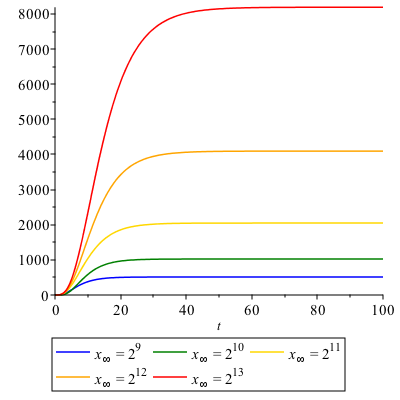
\includegraphics[width=.55\textwidth]{exercises/ex6p1}
	\caption{Plot of x(t) for different $x_\infty$}
	\label{fig:ex6p1}
\end{figure}\\
One can clearly see how the body mass approaches the asymptotic limit $x_\infty$. This stands in contrast to the simple model as the following comparison shows.
Solving the simple differential growth equation for x(t) follows the same procedure as the advanced one and will therefore not be shown in detail. The result is:

\begin{equation}
    x_{init}(t)=\dfrac{1}{(-Abt+At+c)^{\tfrac{1}{b-1}}}
\end{equation}
Plotting the two functions yields

\begin{figure}[h!]
\centering
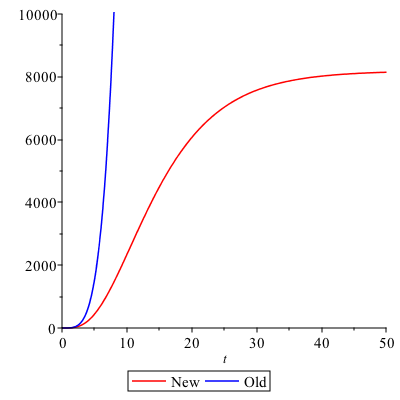
\includegraphics[width=.6\textwidth]{exercises/ex6p2}
	\caption{Illustration of differences between the initial and the new growth rate in a loglogplot}
	\label{fig:ex6p2}
\end{figure}
This plot confirms that the new model is more realistic. While the initial model assumes an exponential growth the continues forever, the updated model shows how the body mass is limited by the maximum size $x_\infty$.
\subsection{The new abundance function}\label{sec:Ex6D}
Since it is not only interesting to know how the body mass of an individual fish develops over time, but also how a stock develops as a whole, one has
to investigate the abundance function that has already been treated in part 1) of this report. The new abundance function is derived by solving the stationary
conservation equation (4) with the new growth function: 

\begin{equation}
    n_{new}(x)=cx^{\dfrac{a+a_F}{x^{A(b-1)}}}(x^b-xx_\infty^{b-1})^{-\tfrac{b-1+a+a_F}{b-1}}
\end{equation}
For clarity, the initial abundance function is stated:

\begin{equation}
    n_{init}(x)=cx^{-b-a-a_Fb}
\end{equation}
The main difference between the two abundance functions is that $n__new(x)$ depends on $x_\infty$. This creates an asymptotic limit for $x -> x_\infty$ as this investigation of the term $(x^b-xx_\infty^{b-1}$ shows:

\begin{equation}
    x\rightarrow x_\infty: x_\infty^b-x_\infty x_\infty^{b-1}=x_{\infty}^b-x_{\infty}^b=0
\end{equation}
Since this term is a factor in $n_{new}(x)$, we can conclude that:

\begin{equation}
    n_{new}(x)\rightarrow0 \textrm{ as } x\rightarrow x_\infty
\end{equation}
Interpreting this biologically, one can say that there are virtually no fish that ever reach a size of $x_\infty$ which is a good representation of reality. This is certainly not the case for the simple model. A plot of the two abundance functions emphasizes the difference between the two.

\begin{figure}[h!]
\centering
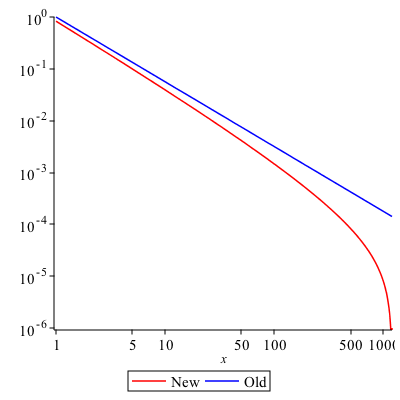
\includegraphics[width=.6\textwidth]{exercises/ex6p3}
	\caption{Illustration of differences between the initial and the new abundance in a loglogplot}
	\label{fig:ex6p3}
\end{figure}\\

%===============================APPENDICES===========================================%

%Appendix A
\cleardoublepage

\appendix
\section{Derivation of the conservation equation}\label{a:calcEx1a}
The differential equations is stated as:
\begin{equation}\label{eq:a1ori}
	\dfrac{\md Ax^{\tfrac{3}{4}}n(x)}{\md x} = -aAx^{\tfrac{3}{4}-1}n(x)
\end{equation}\\
First it is seen that $A$ can be divided out:
\begin{align}
	\dfrac{\md Ax^{\tfrac{3}{4}}n(x)}{\md xA} = \dfrac{-aAx^{\tfrac{3}{4}-1}n(x)}{A}\\
	\dfrac{\md x^{\tfrac{3}{4}}n(x)}{\md x} = -ax^{\tfrac{-1}{4}}n(x) \label{eq:a1aout}
\end{align}\\
The derivative will first be solved using the \textit{product rule}:
\begin{equation}
	\dfrac{\md x^{\tfrac{3}{4}}n(x)}{\md x} = \tfrac{3}{4}x^{\tfrac{-1}{4}}n(x)+x^{\tfrac{3}{4}}\dfrac{\md n(x)}{x}
\end{equation}\\
Substituting this in equation \ref{eq:a1aout} the equation now looks like:
\begin{equation}
\tfrac{3}{4}x^{\tfrac{-1}{4}}n(x)+x^{\tfrac{3}{4}}\dfrac{\md n(x)}{x} = -ax^{\tfrac{-1}{4}}n(x)\\
\end{equation}\\
$\dfrac{\md n(x)}{x}$ can now be isolated by subtracting $\tfrac{3}{4}x^{\tfrac{-1}{4}}n(x)$ from both sides and divide through with $x^{\tfrac{3}{4}}$:
\begin{equation}
\dfrac{\md n(x)}{x} = -ax^{-1}n(x)-\tfrac{3}{4}x^{-1}n(x)=n(x)x^{-1}(\tfrac{-3}{4}-a)\\
\end{equation}\\
It is known that when differentiating certain equation, that the differential is found be multiplying the
function with the power and subtracting one from the power ie. $\dfrac{\md x^{a}}{x}=ax^{a-1}$. Using
this approach, it is seen that $n(x)$ is multiplied with $x^{-1}$ which is equivalent to subtracting one
from the power of a function only containing an x to the power of something multiplied with a constant.
Given this the power of x, must be the constant the function itself is multiplied with which in the case
of the differential is $\tfrac{-3}{4}-a)$. A qualified guess for a solution will the be:
\begin{equation}\label{eq:a:nx}
	n(x) = cx^{\tfrac{-3}{4}-a} \qquad \textrm{where } c \in \mathbb{R}
\end{equation}\\
To check if this is a valid solution one can substitute the solution for $n(x)$ in the original equation given in equation \ref{eq:a1ori}. As this is rather tedious to do by hand the following equations are done in Maple:
\begin{align}
\dfrac{\md Ax^{\tfrac{3}{4}}n(x)}{\md x} = aAx^{-1-a}c\\
	-aAx^{\tfrac{3}{4}-1}n(x) = aAx^{-1-a}c
\end{align}

This proves that the found solution for $n(x)$ indeed is a valid solution.\\
\\
\textbf{\hyperref[jmp:a:calcEx1a]{Jump back }}

\newpage
% Appendix B
\section{Plot of the biomass as a function of two variables}\label{a:biomassPlot}
The equation for the biomass is given as an integral:
\begin{equation}
    \int_{x}^{xc}n(x)xdx
\end{equation}
Or given the equation found for n(x) in formula \ref{eq:Ex1n} and the given value of $a=0.3$:
\begin{equation}
    \int_{x}^{xc}cx^{\tfrac{9}{20}}xdx
\end{equation}
This integral yields a function of two variables:
\begin{equation}\label{eq:biomass2v}
biomass(x,c) = -{\frac {20\,c}{19} \left( {x}^{{\frac{19}{20}}}- \left( xc \right) ^{{\frac{19}{20}}} \right) }
\end{equation}
Below in fig. \ref{fig:a2p1} is this functions shown combined with 3 lines of constant c-values.
\begin{figure}[H]
\centering
    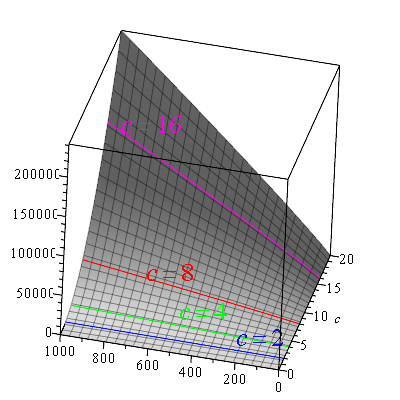
\includegraphics[width=.75\textwidth]{appendices/a2p1.png}
    \caption{Plot of the biomass from x to xc. The lines correspond different c-constants, namely; blue is 5, green is 10 and red is 20}
    \label{fig:a2p1}
\end{figure}\\
From the plot it can be seen that the c-value has a great effect to the biomass; at least from x-values between 0 and 100.\\
\\
\textbf{\hyperref[jmp:a:biomassPlot]{Jump back }}

\newpage

% Appendix C
\section{Approximation of difference in biomass}\label{a:biomassDifApprox}
The difference in two biomasses with equal x-values is given by (from equation \ref{eq:biomass2v}): 

\begin{equation}
	 -{\frac {20c_{big}}{19} \left( {x}^{{\frac{19}{20}}}- \left( xc_{big} \right) ^{{\frac{19}{20}}} \right) } = k\cdot \left(-{\frac {20c_{small}}{19} \left( {x}^{{\frac{19}{20}}}- \left( xc_{small} \right) ^{{\frac{19}{20}}} \right) }\right) 
\end{equation}\\
Here $k$ is the constant corresponding to the difference between them. To find $k$ it will first be isolated:

\begin{equation}
	k = \dfrac{-{\frac {20c_{big}}{19} \left( {x}^{{\frac{19}{20}}}- \left( xc_{big} \right) ^{{\frac{19}{20}}} \right) }}{-{\frac {20c_{small}}{19} \left( {x}^{{\frac{19}{20}}}- \left( xc_{small} \right) ^{{\frac{19}{20}}} \right) }}
\end{equation}
This can be simplified to:
\begin{equation}
	k = \dfrac{c_{big}\left(-{x}^{{\frac{19}{20}}}+\left( xc_{big} \right) ^{{\frac{19}{20}}} \right) }{c_{small} \left(- {x}^{{\frac{19}{20}}}+\left( xc_{small} \right) ^{{\frac{19}{20}}} \right)}
\end{equation}
Given the approximation that $\dfrac{19}{20} \approx 1$ the equation becomes:
\begin{equation}
	k = \dfrac{c_{big}\left(xc_{big}-x\right) }{c_{small} \left( xc_{small}-x\right)}
\end{equation}
Dividing through with x yields:
\begin{equation}\label{eq:a:2:kapproxSmall}
	k = \dfrac{c_{big}\left( c_{big}-1\right) }{c_{small} \left( c_{small}-1\right)}
\end{equation}

Given that $c_{big}$ is the double of $c_{small}$ the equation be written as:
\begin{equation}\label{eq:a:2:kapproxDoubleSmall}
	k = \dfrac{2c_{small}\left(2c_{small}-1\right) }{c_{small} \left( c_{small}-1\right)} = \dfrac{4c_{small}-2}{c_{small}-1}
\end{equation}
\subsection{Large c-values}\label{a:sub:largeCvalues}

For large c-values, $c \gg 1 $, the expressions $\left(c_{big}-1\right)$ and $\left(c_{small}-1\right)$ simply becomes $c_{big}$ and $c_{big}$ respectively. This yields the approximations:
\begin{equation}\label{eq:a:2:kapproxSmall}
	k = \dfrac{c_{big}^2}{c_{small}^2}
\end{equation}
Similar for the doubling approximation in equation \ref{eq:a:2:kapproxDoubleSmall} k simply becomes:
\begin{equation}\label{eq:a:2:kapproxSmall}
	k = 4
\end{equation}
So a doubling in a large c-value will approximately result in a quadrupling in biomass.\\
\\
\textbf{\hyperref[jmp:a:biomassDifApprox]{Jump back }}

\newpage
% Appendix d
\section{Proof of the approximation of the cohort biomass}\label{a:proofBiomassCohort}
The assumptions is that the following is true:
\begin{equation}
  \int_{x}^{x+\tfrac{\md x(t)}{\md t}\cdot\Delta t} n(\xi)\cdot\xi \md \xi \approx n(x)x\dfrac{\md x(t)}{\md t}\Delta T
\end{equation}\\
To prove this one will look at the left hand side of the equation. First $n(\xi)$ is substituted for the known expression of n(x) found in \hyperref[a:calcEx1a]{Appendix \ref{a:calcEx1a}}, equation \ref{eq:a:nx}:
\begin{equation}
    	\int_{x}^{x+\tfrac{\md x(t)}{\md t}\cdot\Delta t} c\cdot\xi^{-(\tfrac{3}{4}+a)}\cdot\xi \md \xi
\end{equation}\\
$\xi$ can be displayed by adding 1 to the power:
    \begin{equation}
    	\int_{x}^{x+\tfrac{\md x(t)}{\md t}\Delta t} c\cdot\xi^{-(\tfrac{3}{4}+a)+1} \md \xi = \int_{x}^{x+\tfrac{\md x(t)}{\md t}\Delta t} c\cdot\xi^{(\tfrac{1}{4}-a)} \md \xi
\end{equation}\\
The integrated function is then:

\begin{equation}
	\left[\dfrac{c\cdot\xi^{(\tfrac{1}{4}-a)+1}}{\tfrac{1}{4}-a+1}\right]_x^{x+\tfrac{\md x(t)}{\md t}\Delta t} = \left[\dfrac{c\cdot\xi^{(\tfrac{5}{4}-a)+1}}{\tfrac{5}{4}-a}\right]_x^{x+\tfrac{\md x(t)}{\md t}\Delta t} 
\end{equation}\\
Now the limits are substituted to solve:

\begin{equation}
	\left(
	    \dfrac{c\cdot\left(
	        x+\tfrac{\md x(t)}{\md }\Delta t
	    \right)^{\tfrac{5}{4}-a}}{\tfrac{5}{4}-a}
	\right)-\left(
	    \dfrac{cx^{\tfrac{5}{4}-a}}{\tfrac{5}{4}-a}
	\right)
\end{equation}
It will be assumed that the a-value is 0.3:

\begin{equation}
	\left(
	    \dfrac{c\cdot\left(
	        x+\tfrac{\md x(t)}{\md }\Delta t
	    \right)^{0.95}}{0.95}
	\right)-\left(
	    \dfrac{cx^{0.95}}{0.95}
	\right)
\end{equation}
Taking the common factor outside the brackets:

\begin{equation}\label{eq:a:2:preapprox}
    \dfrac{c}{0.95}\left(
        \left(
            x+\tfrac{\md x(t)}{\md }\Delta t
        \right)^{0.95}-x^{0.95}
    \right)
\end{equation}
Next, three approximations are made:

\begin{gather}
    \dfrac{c}{0.95}\approx c\\
    \left(
            x+\dfrac{\md x(t)}{\md }\Delta t
        \right)^{0.95} \approx
    \left(
        x+\dfrac{\md x(t)}{\md }\Delta t
    \right)\\
    x^{0.95} \approx x
\end{gather}
Given these approximation the formula \ref{eq:a:2:preapprox} can be estimated to:

\begin{equation}
	\dfrac{c}{0.95}\left(
        \left(
            x+\dfrac{\md x(t)}{\md }\Delta t
        \right)^{0.95}-x^{0.95}
    \right)
    \approx
    c\left(   
        x+\dfrac{\md x(t)}{\md }\Delta t-x
    \right)
\end{equation}
Which can be simplified to:

\begin{equation}\label{eq:a:2:approxDone}
	c\dfrac{\md x(t)}{\md }\Delta t
\end{equation}
Now taking a look at the original approximation:

\begin{equation}
	n(x)x\dfrac{\md x(t)}{\md t}\Delta T
\end{equation}
Again with an a-value of 0.3 n(x) can be substituted with n(x) found in \hyperref[a:calcEx1a]{Appendix \ref{a:calcEx1a}} equation \ref{eq:a:nx}:

\begin{equation}
	c\codt x^{-1.05}x\dfrac{\md x(t)}{\md t}\Delta T = c\codt x^{-0.05}\dfrac{\md x(t)}{\md t}\Delta T
\end{equation}
Approximating that $x^{-0.05}\approx x^0=1$ the function becomes:

\begin{equation}
    c\dfrac{\md x(t)}{\md }\Delta t
\end{equation}
This is the same result as achieved through approximating our integral as seen in equation \ref{eq:a:2:approxDone}.\\
\\
\textbf{\hyperref[jmp:a:proofBiomassCohort]{Jump back }}

\newpage
% Appendix E
\section{Piece wise abundance function}\label{a:abundancepiecewise}
The piece wise mortality is given as;
\begin{equation}\label{eq:a:pBC:1}
\mu(x) =
       \left\{
        \begin{array}{ll}
              \alpha x^{b-1} & x_0 < x < x_F \\
              (\alpha+\alpha_F)x^{b-1} &  x\geq x_F \\
        \end{array} 
\right.
\end{equation}
First the function can be re-written in terms of a and A given that;

\begin{align}
    \alpha = aA\\
    \alpha_F = a_FA\\
    b=\dfrac{3}{4}
\end{align}
then;

\begin{equation}\label{eq:a:pBC:2}
\mu(x) =
       \left\{
        \begin{array}{ll}
              aA x^{\tfrac{3}{4}-1} & x_0 < x < x_F \\
              (aA+a_FA)x^{\tfrac{3}{4}-1} &  x\geq x_F \\
        \end{array} 
\right.
\end{equation}
The differential equation is the function given as;

\begin{equation}
	\dfrac{\md Ax^{\tfrac{3}{4}}n(x)}{\md x} = -\mu(x)n(x)
\end{equation}
A piecewise function can be split up into two differential equations;

\begin{equation}\label{eq:a:pBCeq1}
	\dfrac{\md Ax^{\tfrac{3}{4}}n(x)}{\md x} = -aA x^{\tfrac{3}{4}-1}n(x)
\end{equation}
and

\begin{equation}\label{eq:a:pBCeq2}
	\dfrac{\md Ax^{\tfrac{3}{4}}n(x)}{\md x} = -(aA+a_FA)x^{\tfrac{3}{4}-1}n(x)
\end{equation}
Noticing that \hyperref[eq:a:pBCeq1]{equation \ref{eq:a:pBCeq1}} is identical to that in \hyperref[a:calcEx1a]{Appendix \ref{a:calcEx1a}}. The solution to that equation is then;

\begin{equation}
	n(x) = c_1x^{\tfrac{-3}{4}-a} \qquad \textrm{where } c_1 \in \mathbb{R}
\end{equation}\\
For \hyperref[eq:a:pBCeq2]{equation \ref{eq:a:pBCeq2}} the approach is identical. rewriting $-(aA+a_FA)$ to $-A(a+a_F)$ one can substitute $a+a_F$ with k. Now the following equation has been obtained;

\begin{equation}
	\dfrac{\md Ax^{\tfrac{3}{4}}n(x)}{\md x} = -kA x^{b-1}n(x)
\end{equation}
This equation is identical with \hyperref[eq:a:pBCeq1]{equation \ref{eq:a:pBCeq1}} just with the constant k instead of a. Therefore the solution is given as,

\begin{equation}
	n_1(x) = c_2x^{\tfrac{-3}{4}-k} \qquad \textrm{where } c_2 \in \mathbb{R}
\end{equation}
Now replacing $a+a_F$ with k the function becomes:

\begin{equation}
	n_2(x) = c_2x^{\tfrac{-3}{4}-a-a_F} \qquad \textrm{where } c_2 \in \mathbb{R}
\end{equation}
As this is a piecewise function; one condition is known. For the function to be continuous then they must be equal in the point $x_F$: 

\begin{align}
	c_1x^{\tfrac{-3}{4}-a} = c_2x^{\tfrac{-3}{4}-a-a_F}
\end{align}
Now it is possible to solve for either $c_1$ or $c_2$. In this report the equation is solved for $c_2$ for consistency. $c_2$ is then isolated,

\begin{align}
	c_2 = c_1\dfrac{x^{\tfrac{-3}{4}-a}}{x^{\tfrac{-3}{4}-a-a_F}} = c_1 x^{\tfrac{-3}{4}-a-(-\tfrac{-3}{4}-a-a_F)}=c_1x^{a_F}
\end{align}
Now substituting $c_2$ and introducing c as, $c=c_1$ for this expression one can write n(x) as a piece wise function:

\begin{equation}
    n(x) =
       \left\{
        \begin{array}{ll}
              cx^{-b-a} & x_0 < x < x_F \\
              x_F^{a_F}cx^{-b-a-a_F} & x_F\leq x \\
        \end{array} 
\right.
\end{equation}
\\
\\
\textbf{\hyperref[jmp:a:abundancepiecewise]{Jump back }}

\newpage
% Appendix F
\section{Function for the yield}\label{a:yieldFunction}
With the function of,
\begin{equation}
    \int_{x_{F}}^{x_{\infty }}\!{x_{F}}^{a_{F}}c{x}^{-b-a-a_{F}}x\alpha_{F
}\,{x}^{b-1}\,{\rm d}x
\end{equation}
When the standard values are substituted in it becomes,
\begin{equation}
   \int_{x_{F}}^{x_{\infty }}\!8\,{x_{F}}^{a_{F}}{x}^{- \frac{3}{4}-0.3
a_{F}}{x}^{3/4}\alpha_{F}\,{\rm d}x
\end{equation}
Now simplifying the x terms,
\begin{equation}
    \int_{x_{F}}^{x_{\infty }}\!8\,{x_{F}}^{a_{F}}{x}^{- 0.3-a_{F}}\alpha_
{F}\,{\rm d}x
\end{equation} and the indices,
\begin{equation}
\int_{x_{F}}^{x_{\infty }}\!8\,{x_{F}}^{a_{F}}{x}^{-3/10-a_{F}}\alpha_
{F}\,{\rm d}x
\end{equation}
The coefficient can be taken out as they are constants, for ease of viewing,
\begin{equation}
    8\,{x_{F}}^{a_{F}}\alpha_{F}\,\int_{x_{F}}^{x_{\infty }}\!{x}^{-3/10-a
_{F}}\,{\rm d}x
\end{equation}
Integrating this function yields the following result,
\begin{equation}
    8x_{F}^{\alpha_{F}}\cdot\left[\dfrac{x^{\dfrac{-3}{10}-\alpha_{F}+1}}{-\dfrac{3}{10}-\alpha_{F}+1}\right]_{x_{F}}^{x_{\infty}}
\end{equation}
The upper limit, $ x_{\infty } $ will be taken to be 1000,
\begin{equation}
    8\,{x_{F}}^{a_{F}}\alpha_{F}\cdot\left( \left( \dfrac{1000^{\dfrac{-3}{10}-\alpha_{F}+1}}{-\dfrac{3}{10}-\alpha_{F}-1} \right) - \left( \dfrac{x_{F}^{-\dfrac{3}{10}-\alpha_{F}-+1}}{-\dfrac{3}{10}-\alpha_{F}+1} \right) \right)
\end{equation}
Simplifying the fractions,
\begin{equation}
    8\,{x_{F}}^{a_{F}}\alpha_{F}\cdot \left( \dfrac{1000^{\dfrac{-3}{10}-a_{F}+1}-x_{F}^{-\dfrac{3}{10}-a_{F}+1}}{-\dfrac{3}{10}-a_{F}+1} \right)
\end{equation}
Now the terms involving $X_{F}$,
\begin{equation}
    (8\cdot\alpha_{F})\cdot \left( \dfrac{x_{F}^{a_{F}}\cdot1000^{-\dfrac{3}{10}-a_{F}+1}-x_{F}^{-\dfrac{3}{10}+1}}{-\dfrac{3}{10}-a_{F}+1} \right)
\end{equation}
and further simplifying the rest of the terms,
\begin{equation}\label{eq:fref}
    (8\cdot\alpha_{F})\cdot\left( \dfrac{x_{F}^{a_{F}}\cdot1000^{\dfrac{7}{10}-a_{F}}-x_{F}^{\dfrac{7}{10}}}{\dfrac{7}{10}-a_{F}} \right)
\end{equation}
When equation \ref{eq:fref} is multiplied by 10 and simplified one final time, it becomes
\begin{equation}
\begin{aligned}
&=\dfrac{\left(80\cdot\alpha_{F}\right)\cdot\left( 1000^{\dfrac{7}{10}-a_{F}}\cdot x_{F}^{\dfrac{7}{10}}\right)}{10\left(\dfrac{7}{10}-a_{F}\right)}\\
&=80\,{\frac {\alpha_{F} \left( {1000}^{{\frac{7}{10}}-a_{F}}{x_{F}}^{a_{F}}-{x_{F}}
^{{\frac{7}{10}}} \right)
}{7-10\,a_{F}}}
\end{aligned}
\end{equation}\\
\\
\textbf{\hyperref[jmp:a:yieldFunction]{Jump back }}

\newpage
% Appendix G
\section{Proof of fishing strategy}\label{a:fishingStrategy}
The equation given by, 
\begin{equation}
    80\,{\frac {\alpha_{F}}{10\,\alpha_{F}-7} \left( {x_{F}}^{{\frac{7}{10
}}}- 125.89\,{{\rm e}^{- 6.9078\,\alpha_{F}}}{x_{F}}^{\alpha_{F}}
 \right) }
\end{equation}
Shall be investigated.

First, the terms containing powers of $\alpha_{F}$ will be examined.\\ 
$x_{F}^{\alpha_{F}}$ will clearly become larger as $\alpha_{F}$ approaches $\infty$, furthermore $\dfrac{125.89}{\rm{e}^{6.9079\cdot\alpha_{F}}}$  $\rightarrow 0$  as  $\alpha_{F} \rightarrow \infty$. \\\\
As such, 
\begin{align*}
    125.89\,{{\rm e}^{- 6.9078\,\alpha_{F}}}{x_{F}}^{\alpha_{F}}
\end{align*}
can be omitted for large values of $\alpha_{F}$ and now the term that is left can be further investigated upon,
\begin{equation}
    \dfrac{80\cdot\alpha_{F}x_{F}^{7/10}}{10\alpha_{F}-7}
\end{equation}
As $\alpha_{F}$ becomes larger, the (-7) term in the denominator becomes insignificant. Thus we are left with,
\begin{align*}
    \dfrac{80\alpha_{F}x_{F}^{7/10}}{10\alpha_{F}}
\end{align*}
Simplifying,
\begin{equation}
    \dfrac{8\cdot\alpha_{F}\cdot x_{F}^{7/10}}{\alpha_{F}}
\end{equation}
Hence, as $\alpha_{F}$ increases, the value increases to a point where it only depends on $x_{F}$.\\\\
Furthermore, in,
\begin{equation}
    125.89\cdot\rm{e}^{-6.9078\alpha_{F}}\cdot x_{F}^{\alpha_{F}}
\end{equation}
when $\alpha_{F}$ increases, the term becomes bigger until $125.89\cdot x_{F}^{\alpha_{F}}$ is overtaken by the increasing rate of $ \rm{e}^{-6.9078\cdot\alpha_{F}}$. This power has the larger value, therefore it will begin to make the whole term tend towards 0 which is when the limit will be reached. \\
\\
\textbf{\hyperref[jmp:a:fishingStrategy]{Jump back }}

\newpage
% Appendix H
\section{Derivation of the abundance given a fishing mortality that is constant with size}\label{a:3extra1nx}
The fishing mortality is (given that $\alpha=aA$:

\begin{equation}
    \mu =
       \left\{
        \begin{array}{ll}
              a\cdot A\cdot x^{b-1} & x < x_F \\
              (a\cdot A)\cdot x^{b-1}+\mu_{F} & x\geq x_F \\
        \end{array} 
        \right.
\end{equation}
Now one can split this into two equations; one for each function in the piece wise function. After that one can solve the differential equation for n(x):
 
\begin{equation}
	\dfrac{\md Ax^{b}n(x)}{\md x} = -\mu_i(x)n(x)
\end{equation}
For $\mu_1(x)=a\cdot A\cdot x^{b-1}$ the answer is already calculated in \hyperref[a:calcEx1a]{Appendix \ref{a:calcEx1a}}

\begin{equation}
    n_1(x)=c_1x^(-b-a)
\end{equation}
The second equation where $\mu_2(x)=a\cdot A\cdot x^{b-1}+\mu_{F}$ can be written as:

\begin{equation}
	\dfrac{\md Ax^{b}n(x)}{\md x} = -((a\cdot A)\cdot x^{b-1}+\mu_{F})n(x)
\end{equation}
Now the product rule can be used to find the derivative of $Ax^bn(x)$

\begin{equation}
    Ax^b\dfrac{\md n(x)}{\md x} + n(x)bAx^{b-1} = -((a\cdot A)\cdot x^{b-1}+\mu_{F})n(x)
\end{equation}
Solving for $\dfrac{\md n(x)}{\md x}$:

\begin{equation}
    \dfrac{\md n(x)}{\md x} = \dfrac{-(a\cdot A)\cdot x^{b-1}+\mu_{F})n(x)-n(x)bAx^{b-1}}{Ax^b}
\end{equation}
The common factor n(x) can be taken out:

\begin{equation}
    \dfrac{\md n(x)}{\md x} = \dfrac{n(x)(-a\cdot A\cdot x^{b-1}-\mu_{F}-bAx^{b-1})}{Ax^b}
\end{equation}
The equation can be rearranged to form a linear differential equation with q(x) = 0:

\begin{equation}
    \dfrac{\md n(x)}{\md x}-n(x)\dfrac{(-a\cdot A\cdot x^{b-1}-\mu_{F}-bAx^{b-1})}{Ax^b}=0
\end{equation}

Now using the \textit{Solution Formula for First-Order Linear Equation}\footnote{The Solution Formula for First-Order Linear Equation is introduced in eNote 11, theorem 11.6 with different constants.}:

For a first order linear homogeneous differential equation in the form,

\begin{equation}
	n'(x)+p(x)n(x) = 0
\end{equation}
one would have the solution:

\begin{equation}\label{eq:difeqsol}
	n(x)=\me^{-P(x)}
\end{equation}
Now identifying p(x) as:

\begin{equation}
	-\dfrac{(-a\cdot A\cdot x^{b-1}-\mu_{F}-bAx^{b-1})}{Ax^b}
\end{equation}
One can now find the indefinite integral of p(x) to find P(x):

\begin{equation}
	P(x) = \int -\dfrac{(-a\cdot A\cdot x^{b-1}-\mu_{F}-bAx^{b-1})}{Ax^b}\md x
\end{equation}
This can be expressed as:

\begin{equation}
	P(x) = \int\dfrac{aAx^{b-1}}{Ax^b}+\dfrac{\mu_F}{Ax^b}+\dfrac{bAx^{b-1}}{Ax^b}\md x
\end{equation}
Simplified to:

\begin{equation}
	P(x) = \int ax^{-1}+\dfrac{\mu_Fx^{-b}}{A}+bx^{-1}\md x
\end{equation}
Now the integral can be calculated:

\begin{equation}
	P(x) = a\ln(x)+\dfrac{\mu_Fx^{-b+1}}{A(1-b)}+b\ln(x)
\end{equation}
Given the solution given in \hyperref[eq:difeqsol]{equation \ref{eq:difeqsol}} the solution can be found as:

\begin{equation}
    c\exp(a\ln(x)+\dfrac{\mu_Fx^{-b+1}}{A(1-b)}+b\ln(x))
\end{equation}
Breaking the exponentials so one can simplify:

\begin{equation}
	c\me^{-a\ln(x))}\me^{-\tfrac{\mu_Fx^{-b+1}}{A(1-b)}}\me^{-n\ln(x)}
\end{equation}
This can be simplified further as $a\ln(x)=ln{x^a}$ and $\me^{ln(x)}=x$:

\begin{equation}
    cx^{-a}\cdot x^{-b}\cdot\me^{-\tfrac{\mu_Fx^{-b+1}}{A(1-b)}}
\end{equation}
This can be simplified one last time tp obtain the final solution:

\begin{equation}
    cx^{-a-b}\cdot\exp\left(-\tfrac{\mu_Fx^{-b+1}}{A(1-b)}\right)
\end{equation}\\
\\
\\
\textbf{\hyperref[jmp:a:3extra1nx]{Jump back }}


\newpage
\section{Derivation of the population growth rate, \textit{r}}\label{a:derivation_r}
% Appendix I
The derivation will be based on the initial conditions,
\begin{equation}
    R=\epsilon\,g \left( x_{m} \right) n \left( x_{m},t \right) x_{m}
\end{equation}
\begin{equation}
    R=g \left( x_{0} \right) n \left( x_{0},t \right) x_{0}
\end{equation}
These expressions can be set equal to each other,
\begin{equation}
    \epsilon\,g \left( x_{m} \right) n \left( x_{m},t \right) x_{m}=g \left( x_{0} \right) n \left( x_{0},t \right) x_{0}
\end{equation}
Next, the function expressions will be inserted,
\begin{gather*}
     \epsilon\,g \left( x_{m} \right) {{\rm e}^{rt}}f \left( x_{m} \right) 
x_{m}=g \left( x_{0} \right) {{\rm e}^{rt}}f \left( x_{0} \right) x_{0}\\
\Rightarrow\epsilon\,g \left( x_{m} \right) f \left( x_{m} \right) x_{m}=g
 \left( x_{0} \right) f \left( x_{0} \right) x_{0}
\end{gather*}
After insertion the following equation is achieved,
\begin{equation}
    \epsilon\,A{x_{m}}^{b}{x_{m}}^{-b-a-a_{F}}{{\rm e}^{{\frac {{x_{m}}^{-
b+1}r}{A \left( b-1 \right) }}}}x_{m}=A{x_{0}}^{b}{x_{0}}^{-b-a-a_{F}}
{{\rm e}^{{\frac {{x_{0}}^{-b+1}r}{A \left( b-1 \right) }}}}x_{0}
\end{equation}
The equation shall be simplified and solved for r,
\begin{align*}
    \epsilon\,A{x_{m}}^{b}{x_{m}}^{-b-a-a_{F}}{{\rm e}^{{\frac {{x_{m}}^{-
b+1}r}{A \left( b-1 \right) }}}}x_{m}&=A{x_{0}}^{b}{x_{0}}^{-b-a-a_{F}}
{{\rm e}^{{\frac {{x_{0}}^{-b+1}r}{A \left( b-1 \right) }}}}x_{0}\\
{\frac {\epsilon\,{x_{m}}^{1-a-a_{F}}}{{x_{0}}^{1-a-a_{F}}}}&=\dfrac{\rm{e}^{\frac{x_{0}^{-b+1}}{A(b-1)}}\cdot r}{\rm{e}^{\frac{x_{m}^{-b+1}}{A(b-1)}}\cdot r}\\
\ln  \left( \epsilon\,{x_{m}}^{1-a-a_{F}}{x_{0}}^{-1+a+a_{F}} \right) 
&=\ln  \left( {{\rm e}^{{\frac {{x_{0}}^{-b+1}r}{A \left( b-1 \right) }
}-{\frac {{x_{m}}^{-b+1}r}{A \left( b-1 \right) }}}} \right) 
\end{align*}
Now it is possible to take the r factor out,
\begin{equation}
    \ln  \left( \epsilon\,{x_{m}}^{1-a-a_{F}}{x_{0}}^{-1+a+a_{F}} \right) 
=r \left( {\frac {{x_{0}}^{-b+1}}{A \left( b-1 \right) }}-{\frac {{x_{
m}}^{-b+1}}{A \left( b-1 \right) }} \right) 
\end{equation}
Multiplying with the denominator,
\begin{equation}
    \ln  \left( \epsilon\,{x_{m}}^{1-a-a_{F}}{x_{0}}^{-1+a+a_{F}} \right) 
A \left( b-1 \right) =r \left( {x_{0}}^{-b+1}-{x_{m}}^{-b+1} \right) 
\end{equation}
Now r can be isolated,
\begin{equation}
    {\frac {\ln  \left( \epsilon\,{x_{m}}^{1-a-a_{F}}{x_{0}}^{-1+a+a_{F}}
 \right) A \left( b-1 \right) }{{x_{0}}^{-b+1}-{x_{m}}^{-b+1}}}=r
\end{equation}
And the final equation can be expressed in terms of $x_0$ and $x_m$ 
\begin{equation}\label{eq:appIr}
    r \left( x_{0},x_{m} \right) ={\frac {\ln  \left( \epsilon\,{x_{m}}^{1
-a-a_{F}}{x_{0}}^{-1+a+a_{F}} \right) A \left( b-1 \right) }{{x_{0}}^{
-b+1}-{x_{m}}^{-b+1}}}
\end{equation}
\textbf{\hyperref[jmp:a:derivation_r]{Jump back }}

\newpage
% Section J
\section{Derivation for the size-distribution f(x)}\label{a:derivation_fx}
For this derivation, the equation for growth rate is given by the equation \ref{eq:Ex1g} and the death rate is given by,
\begin{equation}
    \mu =  (\alpha-\alpha_{F]})x^{b-1}
\end{equation}
It is desired to derive f(x) in,
\begin{equation}\label{eq:appJeq}
    \dfrac{\mathrm{d}e^{rt}f(x)}{\mathrm{d}t}+\dfrac{\mathrm{d}g(x)e^{rt}f(x)}{\mathrm{d}x}=\mu(x)e^{rt}f(x)
\end{equation}
Through differentiation, equation \ref{eq:appJeq} becomes,
\begin{equation}\label{eq:appJeq2}
    f \left( x \right) r{{\rm e}^{rt}}+{{\rm e}^{rt}} \left( g \left( x
 \right) {\frac {\rm d}{{\rm d}x}}f \left( x \right) + \left( {\frac 
{\rm d}{{\rm d}x}}g \left( x \right)  \right) f \left( x \right) 
 \right) =-\mu \left( x \right) {{\rm e}^{rt}}f \left( x \right) 
\end{equation}
The $e^{rt}$ terms can be cancelled out so equation \ref{eq:appJeq2} becomes,
\begin{equation}
    f \left( x \right)  r\left(+g \left( x \right) {\frac {\rm d}{{\rm d}x}}f
 \left( x \right) + {\frac {\rm d}{{\rm d}x}}g \left( x
 \right)  f \left( x \right) \right)=-\mu \left( x \right) f \left( x
 \right) 
\end{equation}
Now $mu(x)*f(x)$ may be added to both sides,in order to form a homogeneous equation to solve,
\begin{equation}
        f \left( x \right)  r\left(+g \left( x \right) {\frac {\rm d}{{\rm d}x}}f
 \left( x \right) + {\frac {\rm d}{{\rm d}x}}g \left( x
 \right)  f \left( x \right) \right)+\mu \left( x \right) f \left( x
 \right) =0
\end{equation}
Some re-arranging and simplification yields,
\begin{equation}
    {\frac {\rm d}{{\rm d}x}}f \left( x \right) +{\frac {f \left( x
 \right)  \left( r+{\frac {\rm d}{{\rm d}x}}g \left( x \right) +\mu
 \left( x \right)  \right) }{g \left( x \right) }}=0
\end{equation}
The coefficient for f(x) can now be used to solve the differential equation:
\begin{equation}\label{eq:appJeq3}
    p \left( x \right) ={\frac {r+{\frac {\rm d}{{\rm d}x}}g \left( x
 \right) +\mu \left( x \right) }{g \left( x \right) }}
\end{equation}
Formulating,
\begin{equation}\label{eq:appJfx}
    f(x) = e^{-P(x)}\cdot c
\end{equation}
\begin{equation}\label{eq:appJeq4}
    P(x)=\int p(x)\mathrm{d}x
\end{equation}
Inserting equation \ref{eq:appJeq3} into equation \ref{eq:appJeq4},
\begin{equation}
\begin{aligned}
    \int \!{\frac {r+{\frac {\rm d}{{\rm d}x}}g \left( x \right) +\mu
 \left( x \right) }{g \left( x \right) }}\,{\rm d}x &=\int \!{\frac {r}{g \left( x \right) }}+{\frac {{\frac {\rm d}{{\rm d}
x}}g \left( x \right) }{g \left( x \right) }}+{\frac {\mu \left( x
 \right) }{g \left( x \right) }}\,{\rm d}x\\
 &=\int \!{\frac {r}{g \left( x \right) }}\,{\rm d}x+\ln  \left( g
 \left( x \right)  \right) +\int \!{\frac {\mu \left( x \right) }{g
 \left( x \right) }}\,{\rm d}x\\
 &=r\int \! \left( g \left( x \right)  \right) ^{-1}\,{\rm d}x+\ln 
 \left( g \left( x \right)  \right) +\int \!{\frac {\mu \left( x
 \right) }{g \left( x \right) }}\,{\rm d}x\\
\end{aligned}
\end{equation}
After this simplification, it can now be used in the full equation substituting in the functions of g(x) and $\mu(x)$.
\begin{equation}
\begin{aligned}
&= r\int\dfrac{1}{A\cdot x^{b}}\mathrm{d}x\int\dfrac{A(b+1)x^{b-1}}{A\cdot x^{b}}dx+\int\dfrac{(\alpha+\alpha_{F})x^{b-1}}{A\cdot x^{b}} dx\\
&=\dfrac{r}{A} \int x^{-b}\mathrm{d}x\int\dfrac{A(b+1)x^{b-1}}{A\cdot x^{b}}dx+\dfrac{(\alpha+\alpha_{F})}{A}\int x^{-1} dx
\end{aligned}
\end{equation}
Integrating this becomes,
\begin{equation}\label{eq:appJeq5}
\begin{aligned}
    {\frac {r{x}^{-b+1}}{A \left( -b+1 \right) }}+\ln  \left( A{x}^{b}
 \right) +{\frac { \left( \alpha+\alpha_{F} \right) \ln  \left( x
 \right) }{A}} &= {\frac {r{x}^{-b+1}}{A \left( -b+1 \right) }}+\ln  \left( A \right) +
\ln  \left( {x}^{b} \right) +{\frac { \left( \alpha+\alpha_{F}
 \right) \ln  \left( x \right) }{A}}\\
P(x) &={\frac {r{x}^{-b+1}}{A \left( -b+1 \right) }}+\ln  \left( A \right) +b
\ln  \left( x \right) +{\frac { \left( \alpha+\alpha_{F} \right) \ln 
 \left( x \right) }{A}}\\
 &={\frac {r{x}^{-b+1}}{A \left( -b+1 \right) }}+\ln  \left( A \right) +
\ln  \left( x \right)  \left( b+{\frac {\alpha+\alpha_{F}}{A}}
 \right) 
\end{aligned}
\end{equation}
Thus, P(x) has been found and can now be re-introduced into equation \ref{eq:appJfx}
\begin{equation}
   f(x) = \mathrm{e}^{- \dfrac{r\cdot x^{1-b}}{A(1-b)}}
\end{equation}
This can be split into 2 different exponential variables,
\begin{equation}
    \mathrm{e}^{-\dfrac{r\cdot x^{-b+1}}{A\cdot (1-b)}}\cdot \mathrm{e}^{-\lnb{x})\cdot \left( b+\dfrac{\alpha+\alpha_{F}}{A} \right)}\cdot c
\end{equation}
Using the exponential power rule $x^{a\cdot b }= x^{a^{b}}$,
\begin{equation}
    \me^{-{\dfrac{r\cdot x^{-b+1}}{A\cdot (1-b)}}}\cdot \me^{ln(x)^{-\left( b+\dfrac{\alpha+\alpha_{F}}{A} \right)}}\cdot c 
\end{equation}

Finally, using the fact that $e^{ln(x)}=x$ and that $e^{-ln(A)}\cdot c = C$, because both A and c were arbitary constants.
\begin{equation}
\begin{aligned}
    f(x)&={{\rm e}^{-{\frac {r{x}^{-b+1}}{A \left( -b+1 \right) }}}}{x}^{-b-{\frac {\alpha+\alpha_{F}}{A}}}\\
    &=C{x}^{-b-{\frac {\alpha}{A}}-{\frac {\alpha_{F}}{A}}}{{\rm e}^{{\frac 
{r{x}^{-b+1}}{A \left( b-1 \right) }}}}
\end{aligned}
\end{equation}\\
\\
\textbf{\hyperref[jmp:a:derivation_fx]{Jump back }}


\newpage
% Appendix K
\section{Derivation of the survival}\label{a:survivalDerivation}
The given function is:
\begin{equation}\label{eq:a:survival}
    P_{x_0\rightarrow x} = \exp\left[{-\int_{x_0}^{x}\tfrac{\mu(x)}{g(x)}\md x}\right]
\end{equation}
First one should look at the integral:

\begin{equation}
    {\int_{x_0}^{x}\tfrac{\mu(x)}{g(x)}\md x}
\end{equation}
Given the function for $\mu(x)$ and $g(x)$ from \ref{eq:Ex1mu} or \ref{eq:Ex1g} respectively, one can write:

\begin{equation}
    \dfrac{\mu(x)}{g(x)}=\dfrac{ax^{b-1}}{x^b}=ax^{-1}
\end{equation}
Now for the integral:

\begin{equation}
    \int_{x_0}^{x}ax^{-1}\md x = a\int_{x_0}^{x}x^{-1}\md x
\end{equation}
Calculating the integral yields:

\begin{equation}\label{hej}
    a\int_{x_0}^{x}x^{-1}\md x = a\left[ln(x) \right]_x^{x_0} = a(ln(x_0)-ln(x))
\end{equation}

Inserting this in function \ref{eq:a:survival} gives the function:

\begin{equation}
    P(x_0,x) = \exp({a(ln(x_0)+ln(x))})
\end{equation}
\\
\\
\textbf{\hyperref[jmp:a:survivalDerivation]{Jump back }}

\end{document}
